\chapter{An overview of the Hazel programming environment}
\label{sec:hazel}

Hazel is the reference implementation for the Hazelnut bidirectionally-typed action semantics and the Hazelnut Live dynamic semantics. It is intended to serve as a proof-of-concept of the semantics with static holes that attempt to mitigate the gap problem; however, the implementation is becoming increasingly practical with more recent additions to the language. The reference implementation is an interpreter written in OCaml and transpiled to Javascript using the \mintinline{text}|js_of_ocaml| (JSOO) library \cite{vouillon2014bytecode} so that it may be run client-side in the browser. A screenshot of the reference implementation is shown in \Cref{fig:screenshot-hazel-ui} \cite{HazelDemo2022}. The source code may be found on GitHub \cite{Hazel2022}. Hazel may be characterized as a purely functional, statically-typed, bidirectionally-typed, strict-order evaluation, structured editor programming language.

\section{Motivation for Hazel}
\label{sec:hazel-motivation}

\subsection{The gap problem}
\label{sec:gap-problem}

Programming editor environments aim to provide feedback to a programmer in the form of editor services such as syntax highlighting or language server protocol (LSP) warnings. Live programming environments aim to provide continuous static (static type error) and dynamic (run-time type error) feedback in real-time, allowing for rapid prototyping. However, over the course of the lifetime of a program, the program may enter many edit states when it is \textit{meaningless} (ill-formed or ill-typed).

Editor services can only assign static and dynamic meaning to programs that are statically well-typed and free of dynamic type errors. Some may deploy reduced ad hoc algorithms of meaningless edit states. This means that over the course of editing, the programmer experiences temporal gaps between moments of complete editor services. This is known as the \textit{gap problem} \cite{10.1145/2499370.2462170,conf/popl/HazelnutLive19}.

\subsection{An intuitive introduction to typed expression holes}
\label{sec:typed-holes}

Hazelnut and Hazelnut Live address the gap problem by defining a static and dynamic semantics, respectively, for a small functional programming language extended with typed holes. It is built on top of a \textit{structure editor}, which ensures that a program is always well-formed (syntactically correct) by disallowing invalid edit actions. The Hazelnut action semantics for typed holes ensures that a well-formed program is always well-typed. The Hazelnut Live dynamic semantics defines an encapsulated behavior for type errors, such that evaluation continues ``around'' and captures information about type errors in order to provide dynamic feedback to the programmer.

The Hazelnut Live paper provides the following intuitive understanding of holes.

\begin{displayquote}
  Empty holes stand for missing expressions or types, and non-empty holes operate as ``membranes''
around static type inconsistencies (i.e. they internalize the ``red underline'' that editors commonly display under a type inconsistency).
\end{displayquote}

We have already acknowledged the existence of type holes in dynamically-typed languages and in the \gtclc{}, in which type holes are represented by the type $\gtlch$. This allows unannotated expressions to statically type-check, with the possibility of running into a dynamic type error at runtime.

Some languages also have the concept of expression holes, which allow a program to be well-typed with missing expressions. In Haskell, for example, the special error value \mintinline{haskell}|undefined| always type-checks but will immediately crash the program if it is encountered during evaluation. Haskell also provides the syntax \mintinline{haskell}|_u| for typed expression holes, which provides static type information but will not compile\footnote{We may force this to compile using the \mintinline{text}|-fdefer-type-errors| flag, but then holes will crash when encountered during evaluation similar to \mintinline{haskell}|undefined|.}. Hazelnut Live is the first example of a dynamic semantics that does not consider the evaluation of holes as an exceptional behavior that would crash the program.

In summary, Hazel provides empty type and expression holes, which represent dynamic typing and missing expressions. Nonempty holes are also provided to encapsulate error conditions and provide a well-defined dynamic semantics while providing useful feedback to the user. The dynamic semantics is carefully defined to stop when such indeterminate expressions are encountered, but continue elsewhere (``around'' holes or failed casts) if possible.

\subsection{The Hazel interface}
\label{sec:hazel-interface}

In \Cref{fig:hazel-interface} the web interface for the Hazel live environment is shown. The left panel marked (1) is a informational panel showing the list of keyboard shortcuts to perform actions. Since Hazel is a structured editor, simply typing the program as plaintext will not work; one must use the appropriate shortcuts the construct and edit the program. (2) is the code view. Below the code, a gray box indicates the result of evaluating the expression. The program result updates in real time with every edit action, assuming that evaluation is turned on. (3) is the context inspector, which shows information about a hole if a hole is selected. It shows the hole environment and typing context, followed by the path to the hole and the number of hole instances. In this case, the third hole in the result is selected, in which $x$ has value $3$. Lastly, (4) shows a history of the edit actions. Hovering or clicking on a past edit state will revert the program to that edit state.

\begin{figure}
  \centering
  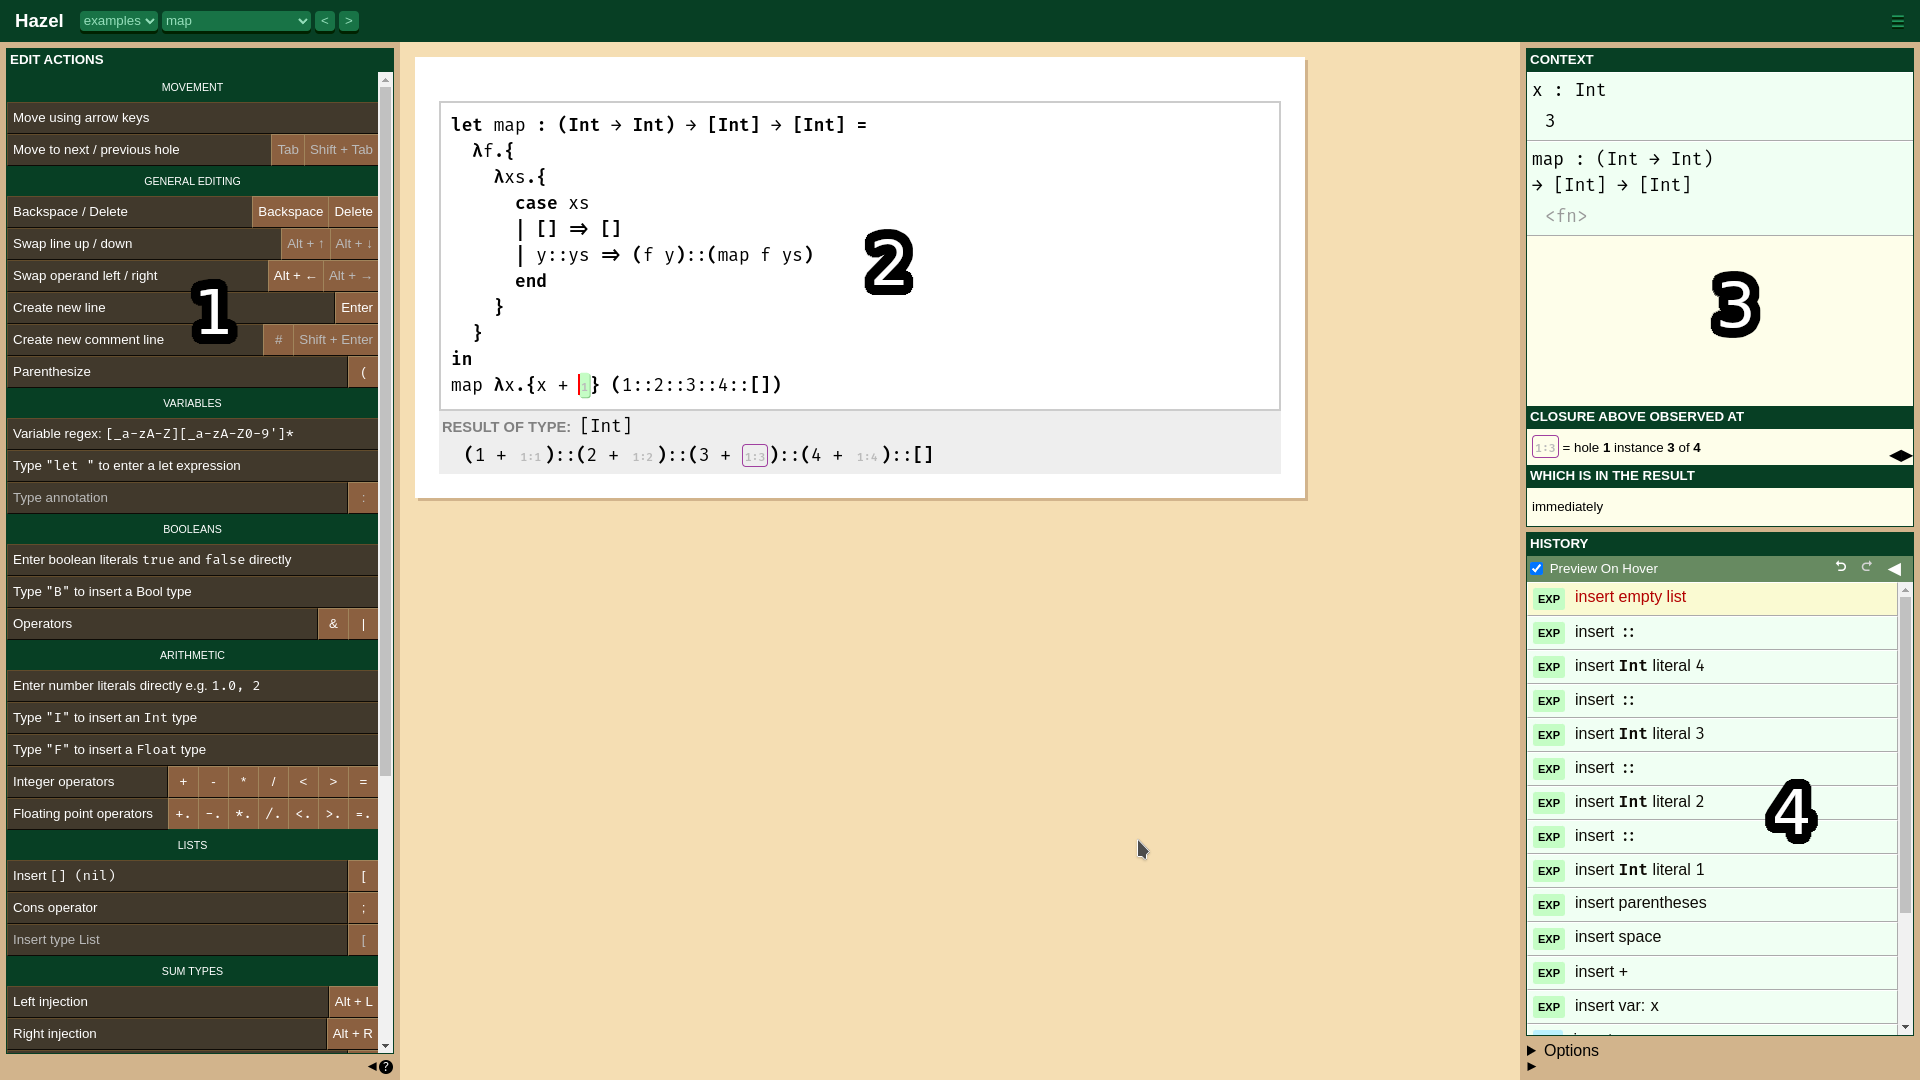
\includegraphics[width=\linewidth]{img/hazel_ui_annot.png}
  \caption{The Hazel interface, annotated}
  \label{fig:hazel-interface}
\end{figure}

\subsection{Implications of Hazel}
\label{sec:hazel-implications}

The main proposed use case of Hazel is its use in programming education, particularly for teaching functional programming, as it provides much useful feedback to the programmer for error conditions, allowing them to focus instead on semantic errors in their algorithm. This is being explored with the Hazel Tutor project \cite{potter2020hazel}.

Another research direction is in its use as a structural and graphical editor. For example, live GUIs \cite{omar2021filling} are being explored to enhance the editing experience by providing live, compositional, graphical interfaces, in addition to the benefits that Hazel's core calculi provide.

The result of a Hazel evaluation may contain holes. The Hazelnut Live paper \cite{conf/popl/HazelnutLive19} suggests the idea of hole-filling: since each hole in the result contains its lexical environment, we may ``resume'' evaluation without restarting evaluation from the beginning if a hole is filled -- this property is similar to that of computational notebooks. The problem with notebook execution is that it is stateful and running operations out-of-order may cause irreversible state changes that cause irreproducible results. On the other hand, resuming an evalution with fill-and-resume will produce the same result as if the program was run ordinarily from start to finish\footnote{This is a property known as \textit{commutativity} and described in \cite{conf/popl/HazelnutLive19}.} while avoiding re-evaluation of previous sections.

\section{Introduction to OCaml and Reason syntax}
\label{sec:ocaml-intro}

Previously, we have been introducing concepts using a pseudo-mathematical notation. When describing Hazel and its implementation, it may be useful to use sample code or pseudocode from the implementation to describe various aspects of Hazel.

Hazel is implemented in Reason (alternatively, ReasonML), which is a dialect of OCaml that offers a JavaScript-like syntax. The Reason code used in this report will be limited to function names and types. Module names are denoted \texttt{PascalCase}, whereas function and type names are \texttt{snake\_case}. Conventionally, OCaml modules that export a type export a single type called \texttt{t}. As an example, \mintinline{ocaml}|DHExp.t| refers to the primarily-relevant type from the \mintinline{ocaml}|DHExp| module, the type that represents internal expressions $d$. On the other hand, \mintinline{ocaml}|Evaluator.evaluate| refers to the \mintinline{ocaml}|evaluate| function in the \mintinline{ocaml}|Evaluator| module. All functions and types will be prefixed with their module names for maximum clarity.

\section{Hazelnut semantics}
\label{sec:hazel-semantics}

Hazel is rigorously defined using a bidirectional semantics. A high-level overview of the foundational papers on Hazelnut (syntax and static semantics) and Hazelnut Live (elaboration and dynamic semantics) is provided here, but a thorough explanation is deferred to the original descriptions \cite{conf/popl/Hazelnut17,conf/popl/HazelnutLive19}.

\subsection{Hazelnut syntax}
\label{sec:hazel-syntax}

The grammar of Hazelnut's external language is reproduced in \Cref{fig:hazelnut-syntax}.

\begin{figure}
  \centering
  \begin{singlespace}
    \begin{align*}
      \tau &::= \tau\to\tau
             \mid b
             \mid \tehole \\
      e &::= c
          \mid x
          \mid\lambda x:\tau.e
          \mid e\ e
          \mid e:\tau
          \mid \hehole
          \mid \hhole{e}
    \end{align*}
  \end{singlespace}  
  \caption{Hazelnut syntax}
  \label{fig:hazelnut-syntax}
\end{figure}

This is very similar to \gtlc{}. The $\gtlch{}$ type is rewritten as $\tehole$ and pronounced the ``hole type.'' An expression form for type ascription is added. Most notably, there is the addition of empty and non-empty expression holes, which are denoted $\hehole$ and $\hhole{e}$, respectively.

\subsection{Hazelnut action and typing semantics}
\label{sec:hazel-statics}

Hazelnut \cite{conf/popl/Hazelnut17} defines a bidirectional typing judgment for the external language. \todo{reproduce this in an appendix} The judgments are very similar to \gtlc{}. Unsurprisingly, hole expressions synthesize the hole type, and they analyze against any type. Note that in the case of a non-empty hole, the encapsulated expression must still synthesize a type, i.e., they are well-typed.

Hazelnut defines an action semantics for the structural editor, which describes the behavior of editing and maneuvering around a program. A program's edit state comprises an external expression with a superimposed cursor. There are four main actions carried out by the user: \texttt{move}, \texttt{construct}, and \texttt{delete}. These actions are described by bidirectionally-typed action judgments that transform a (well-typed) edit state to another (well-typed) edit state. There are a number of metatheorems that enforce desirable properties of action semantics in a structural editor, such as \textit{sensibility} (the result of an action on a well-typed expression is a well-typed expression), \textit{movement erase invariance} (movement actions should not change the external expression, but only the position of the cursor), \textit{reachability} (the cursor should be able to move to any valid location to any other valid location), \textit{constructability} (every valid edit state should be constructable from the initial edit state), \textit{action determinism} (every sequence of edit actions should have only one valid output state), etc. These metatheorems are proved using the Agda theorem proving assistant \cite{agda2017}.

\subsection{Hazelnut Live elaboration judgment}
\label{sec:hazel-elaboration}

\textit{Elaboration} is the process of converting an expression from the external language to the internal language. Notably, both the external and internal languages share the same type system. The internal language and the elaboration process is very similar to the cast calculus \gtclc and the elaboration process from \gtlc.

The elaboration algorithm is also bidirectionally-typed, and thus involves two mutually-recursive judgments: a \textit{synthetic elaboration judgment} $\Gamma^-\vdash e^-\Rightarrow\tau^+\leadsto d^+\dashv\Delta^+$, and an \textit{analytic elaboration judgment} $\Gamma^-\vdash e^-\Leftarrow\tau^-\leadsto d^+:\tau'^+\dashv\Delta^+$.\todo{reproduce elaboration judgments in appendix}

$\Delta$ is the \textit{hole context}, used to store the typing context and actual type of each hole. Each hole (whether in synthetic or analytic position) is recorded in the hole context, and is given the identity mapping as its original environment\footnote{This is amended in this work, in which holes will not initially be given an environment because the environment is not substitution-based.}.

The elaboration judgment will produce as output a type for the internal expression, which may be different from the type of the external expression. In particular, elaborated holes will produce different types depending on whether they are in synthetic or analytic position.

\subsection{Hazelnut Live final judgment and dynamic semantics}
\label{sec:hazel-dynamics}

Hazelnut Live introduces a new $d\textsf{ final}$ judgment for the internal language, used to indicate an irreducible expression. This subsumes the set of fully-evaluated expressions in \gtclc, which include plain values or \textit{boxed values}, values which are casted ``out'' of their original type but not yet casted ``into'' the destination type. However, expressions containing holes also cannot further evaluate and comprise the second class of final expressions: \textit{indeterminate} values.

\todo{reproduce final judgment}

Hazelnut Live defines a small-step semantics for its internal language very similar to that of \gtclc. To avoid the rapid proliferation of rules due to the small-step semantics, a notational convenience called the \textit{evaluation context} $\mathcal{E}$, which recursively evaluates subexpressions. The rules are modified to accomodate indeterminate expressions.

\todo{reproduce small-step semantics in an appendix}

Hazelnut and Hazelnut Live only define rules for the core expression types, and does not define rules for all expression types. For example, fixpoint expressions, \mintinline{ocaml}|let| expressions, and \mintinline{ocaml}|case| expression types are present in Hazel but not discussed in Hazelnut or Hazelnut Live. We follow suit when discussing rules, but will discuss practical concerns that arise with these expression forms.

\subsection{Hole instance numbering}
\label{sec:hole-instance-numbering}

Hazelnut Live introduces \textit{hole instances} with some motivation, but with no details of its implementation. In \Cref{sec:renumbering}, we will motivate hole instances in greater detail, describe the current implementation, and reformulate the problem of hole instance tracking to accomodate environments and memoization.

%%% Local Variables:
%%% mode: latex
%%% TeX-master: "main"
%%% End:
